\documentclass[a4paper,12pt]{article}

\usepackage{amsfonts, amsmath, amssymb, amsthm, dsfont, enumitem, fancyhdr, graphicx}
\usepackage[margin=0.9in, includehead, includefoot, heightrounded]{geometry}
\allowdisplaybreaks
\pagestyle{fancy}
\rhead{Erick Lin}

\newcommand{\norm}[1]{\left\lVert#1\right\rVert}
\newcommand*\dist{\mathop{\!\mathrm{d}}}
\DeclareMathOperator{\im}{Im}
%\let\ker\relax %RedeclareMathOperator
%\DeclareMathOperator{\ker}{Ker}
\renewcommand{\thesubsection}{\arabic{subsection}}
\newcommand*\sq{\mathbin{\vcenter{\hbox{\rule{.3ex}{.3ex}}}}}
\newcommand{\iso}{\approx}
\newtheorem{theorem}{Theorem}
\newtheorem{lemma}[theorem]{Lemma}

\begin{document}

\section*{MATH 6441 -- Midterm Corrections}
\subsection*{Section 2.1}
\begin{enumerate}
    \item
        Let $\varphi : X \to S^1$. Since $\pi_1(X)$ is finite, the image of the induced homomorphism $\varphi_* : \pi_1(X) \to \pi_1(S^1)$ must be a finite subgroup of $\pi_1(S^1) \approx \mathbb{Z}$, the only one that exists of which is the trivial group; in other words, $\varphi_*(\pi_1(X)) = 0$. Because we know that there exists a covering space $p : \mathbb{R} \to S^1$ (defined by $p(s) = (\cos 2\pi s, \sin 2\pi s)$), we have the existence of a lift $\tilde{\varphi} : X \to \mathbb{R}$ of $\varphi$ by the lifting criterion. $\mathbb{R}$ is contractible, and so $\tilde{\varphi}$ is nullhomotopic by some homotopy $h_t$. Then $\varphi$ is also nullhomotopic, by the homotopy $p h_t$.

    \item
        \begin{enumerate}[label=(\alph*)]
            \item
                $X_k$ deformation retracts to a sphere $S^2$ centered at the origin with $2k$ points, the intersection points of $Z_k$ with the sphere, removed. Then this sphere with $2k$ points removed stereographically projects onto the plane $\mathbb{R}^2$ with $2k - 1$ points removed (if we take one of the removed points as the north pole, on which the projection is undefined), which is a homeomorphism. Lastly, the plane with $2k - 1$ points removed deformation retracts onto the wedge sum of $2k - 1$ circles, whose fundamental group is the free group on $2k - 1$ generators. Thus, $\pi_1(X_k)$ is this fundamental group also.
            \item
                $\pi_1(X_1)$ is the free group on $1$ generator, which is just $\mathbb{Z}$. Because $\mathbb{Z}$ is a proper subgroup of the free group on $2k - 1$ generators, the homomorphism $i_* : \pi_1(X_k) \to \pi_1(X_1)$ induced by the inclusion $i : X_k \to X_1$ cannot be injective. Then by Proposition 1.17, $X_1$ does not retract onto $X_k$.
        \end{enumerate}

    \item
        \begin{enumerate}[label=(\alph*)]
            \setcounter{enumii}{1}
            \item
                The normal subgroup generated by $a$ is the set of all elements conjugate to $a$, or of the form $gag^{-1}$, $g \in \langle a, b \rangle$. %; quotienting by this normal subgroup identifies all these conjugate elements to $1$, hence allowing for the assumption that $g = b^n$ for some $n$.
                Hence, $\ker\phi = \langle b^n a b^{-n}, n \in \mathbb{Z} \rangle$, which corresponds to the covering space shown below. \par
                {\centering
                    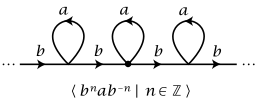
\includegraphics[scale=1]{midterm_3b}
                \\}
                The deck group $G$ consisting of all symmetries of this covering space is isomorphic to $\mathbb{Z}$, and its action on the covering space is the translational symmetry generated by $b$.
        \end{enumerate}

    \item
        Since $L$ is the union of two linked circles, $\mathbb{R}^3 - L$ deformation retracts onto the wedge sum of $S^2$ and a torus $S^1 \times S^1$ separating the linked circles, as shown in the figure below. \par
        {\centering
            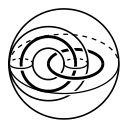
\includegraphics[scale=1]{midterm_4}
        \\}
        Thus (we can use Proposition 1.12 since $S^1$ is path-connected), $\pi_1(\mathbb{R}^3 - L) \approx \pi_1(S^2 \lor (S^1 \times S^1)) \approx \pi_1(S^2) * \pi_1(S^1 \times S^1) \approx \pi_1(S^1) \times \pi_1(S^1) \approx \mathbb{Z} \times \mathbb{Z}$.

\end{enumerate}
\end{document}
